\documentclass[11pt,a4paper]{article}

% ---------- Codifica e lingua ----------
\usepackage[T1]{fontenc}
\usepackage[utf8]{inputenc}
\usepackage[main=italian,provide=*]{babel}

% ---------- Matematica ----------
\usepackage{amsmath,amssymb,amsthm}
\usepackage{mathtools}

% ---------- Impaginazione ----------
\usepackage[a4paper,margin=2.6cm]{geometry}
\usepackage{caption}
\captionsetup{font=small,labelfont=bf,width=.92\linewidth}
\usepackage{booktabs}
\usepackage{enumitem}
\usepackage{placeins}
\usepackage[colorlinks=true,linkcolor=black,citecolor=black,urlcolor=blue!55!black]{hyperref}

% ---------- Grafica ----------
\usepackage{xcolor}
\usepackage{tikz}
\usetikzlibrary{arrows.meta,positioning,calc,matrix,backgrounds,decorations.pathreplacing,fit,shapes.geometric}
\usepackage{pgfplots}
\pgfplotsset{compat=1.18}
\usepackage{nicematrix}

% ---------- Colori ----------
\definecolor{spinup}{HTML}{C24A22}
\definecolor{spindown}{HTML}{2E6FB0}
\definecolor{amber}{HTML}{9A6212}
\definecolor{teal}{HTML}{0F6E56}
\definecolor{blockP}{HTML}{ECECEC}
\definecolor{blockQ}{HTML}{D7EBE4}
\definecolor{blockC}{HTML}{F6E7CC}

% ---------- Macro ----------
\newcommand{\ket}[1]{\lvert #1 \rangle}
\newcommand{\bra}[1]{\langle #1 \rvert}
\newcommand{\braket}[2]{\langle #1 \vert #2 \rangle}
\newcommand{\melem}[3]{\langle #1 \vert #2 \vert #3 \rangle}
\newcommand{\up}{\uparrow}
\newcommand{\dn}{\downarrow}
\newcommand{\dg}{\dagger}
\renewcommand{\vec}[1]{\boldsymbol{#1}}
\newcommand{\sv}{\vec{s}}
\newcommand{\opn}{\hat{n}}
\newcommand{\Heff}{H_{\mathrm{eff}}}

\theoremstyle{definition}
\newtheorem*{nota}{Nota}
\theoremstyle{remark}
\newtheorem*{oss}{Osservazione}

% ---------- Disegno spin ----------
\newcommand{\arrowup}[2]{\draw[spinup,line width=1.2pt,-{Stealth[length=2.4mm,width=2mm]}] (#1,{#2-0.22}) -- (#1,{#2+0.24});}
\newcommand{\arrowdn}[2]{\draw[spindown,line width=1.2pt,-{Stealth[length=2.4mm,width=2mm]}] (#1,{#2+0.22}) -- (#1,{#2-0.24});}

% =====================================================================
\begin{document}

\begin{titlepage}
\centering
\vspace*{2.0cm}
{\Large\scshape Università degli Studi di Parma}\\[0.3cm]
{\large Dipartimento di Scienze Matematiche, Fisiche e Informatiche}\\[2.2cm]
\rule{\linewidth}{0.4pt}\\[0.5cm]
{\LARGE\bfseries Dal modello di Hubbard all'Hamiltoniana di scambio}\\[0.35cm]
{\large\itshape Derivazione completa del dimero di spin di Heisenberg\\ per la simulazione quantistica variazionale (VQE)}\\[0.4cm]
\rule{\linewidth}{0.4pt}\\[1.6cm]

\begin{flushright}
\begin{minipage}{0.5\linewidth}
\begin{flushleft}
\textbf{Materiale di studio}\\
Samuele\\[0.4cm]
\textbf{Relatore}\\
Prof.\ Alessandro Chiesa
\end{flushleft}
\end{minipage}
\end{flushright}

\vfill
{\small Riferimento concettuale: M.~Crippa \textit{et al.}, \textit{Magnetochemistry} \textbf{7}, 117 (2021);\\
materiale del corso ``6 -- Applications''.}\\[0.6cm]
{\small\today}
\end{titlepage}

\tableofcontents
\newpage

\begin{abstract}
\noindent Questo documento ricostruisce in modo \emph{completo e autosufficiente} l'Hamiltoniana di spin
isotropa di tipo Heisenberg che descrive un dimero magnetico, fino alla forma in operatori di Pauli usata
nell'esempio ``VQE on a spin dimer''. Nessun passaggio è dato per acquisito: si verificano le matrici dei
modi fermionici, si calcola l'azione di $H_t$ con tutti i segni di anticommutazione, si deriva la formula
perturbativa del secondo ordine e si valutano esplicitamente i suoi elementi di matrice, si svolge la
diagonalizzazione $2\times2$ (sia per la repulsione $\mathcal P$--$\mathcal Q$ con i suoi $E_\pm$, sia per
l'Hamiltoniana efficace $\mathcal P$--$\mathcal P$), si espandono le approssimazioni indicando i termini
trascurati e il regime di validità, si ricava la mappa sugli operatori di spin che fissa $J=4t^2/U$, e si
deriva infine lo spettro completo del dimero con campo. L'Appendice~\ref{app:spin} richiama l'algebra di
spin-$\tfrac12$ usata nel testo. Ogni passaggio è accompagnato da una figura.
\end{abstract}

% =====================================================================
\section{Inquadramento del sistema}

\subsection{Che cosa è il dimero: una molecola, non due elettroni liberi}

Il dimero di spin \emph{non} descrive due elettroni liberi nello spazio continuo, bensì due
\textbf{centri magnetici localizzati} -- tipicamente due ioni paramagnetici tenuti a posizione fissa
dalla struttura molecolare. Ogni ione porta un elettrone spaiato, cioè uno spin-$\tfrac12$ ben
localizzato sul proprio sito. I gradi di libertà spaziali sono ``congelati'' (l'elettrone resta sul suo
sito); restano dinamici solo gli orientamenti di spin. È il quadro dei \emph{molecular nanomagnets} di
Crippa \textit{et al.}: il dimero ($N=2$) è il mattone elementare di catene e anelli di Heisenberg.

L'accoppiamento $J$ tra i due spin non è un'interazione magnetica diretta tra i momenti (troppo
debole), ma uno \textbf{scambio} mediato da un ponte chimico diamagnetico: il \emph{superscambio}
(Figura~\ref{fig:molecola}).

\begin{figure}[htbp]
\centering
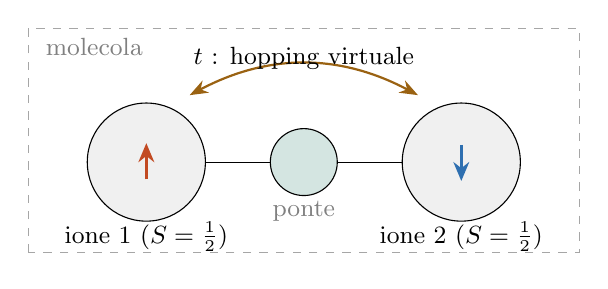
\begin{tikzpicture}[>=Stealth]
  \draw[dashed,gray!70] (-3.5,-1.15) rectangle (3.5,1.7);
  \node[gray,font=\small,anchor=west] at (-3.4,1.46) {molecola};
  \node[circle,draw,fill=gray!12,minimum size=1.5cm] (i1) at (-2,0) {};
  \node[circle,draw,fill=gray!12,minimum size=1.5cm] (i2) at (2,0) {};
  \node[circle,draw,fill=teal!18,minimum size=0.85cm] (br) at (0,0) {};
  \draw (i1) -- (br) -- (i2);
  \arrowup{-2}{0}\arrowdn{2}{0}
  \draw[<->,amber,thick] (-1.45,0.85) to[bend left=28] (1.45,0.85);
  \node[font=\small] at (0,1.32) {$t$ : hopping virtuale};
  \node[gray,font=\small] at (0,-0.62) {ponte};
  \node[font=\small] at (-2,-0.95) {ione 1 ($S=\tfrac12$)};
  \node[font=\small] at (2,-0.95) {ione 2 ($S=\tfrac12$)};
\end{tikzpicture}
\caption{Schema fisico del dimero: due ioni magnetici localizzati, ognuno con un elettrone spaiato
(spin $\up$ e $\dn$), collegati da un ponte diamagnetico attraverso cui agisce il superscambio.}
\label{fig:molecola}
\end{figure}

\subsection{Obiettivo e mappa del documento}
Vogliamo arrivare, motivandola passo per passo, all'Hamiltoniana del documento di riferimento,
\begin{equation}
H = J_x\,X_1X_2 + J_y\,Y_1Y_2 + J_z\,Z_1Z_2 + b\,(Z_1+Z_2),
\label{eq:Hfull}
\end{equation}
nel caso isotropo $J_x=J_y=J_z\equiv J$, capendo \emph{perché} ha questa forma. La Sezione~\ref{sec:hubbard}
deriva l'origine microscopica dello scambio dal modello di Hubbard; la Sezione~\ref{sec:dimero} discute la
forma completa~\eqref{eq:Hfull} con il campo e ne ricava lo spettro. L'Appendice~\ref{app:spin} raccoglie
le convenzioni e i risultati di algebra di spin-$\tfrac12$ usati ovunque nel testo.

\FloatBarrier
% =====================================================================
\section{Origine microscopica dello scambio}
\label{sec:hubbard}

\subsection{Il modello di Hubbard a due siti}

Lo scambio nasce dalla combinazione di repulsione coulombiana e principio di Pauli. Il modello minimo è
quello di Hubbard sul dimero (due siti, un orbitale ciascuno, due elettroni totali, \emph{half-filling}):
\begin{equation}
H = \underbrace{-t\sum_{\sigma}\!\big(c_{1\sigma}^{\dg}c_{2\sigma}+c_{2\sigma}^{\dg}c_{1\sigma}\big)}_{H_t\ \text{(hopping)}}
\;+\;\underbrace{U\big(\opn_{1\up}\opn_{1\dn}+\opn_{2\up}\opn_{2\dn}\big)}_{H_U\ \text{(repulsione on-site)}}.
\label{eq:hubbard}
\end{equation}
Qui $t>0$ è l'ampiezza di salto tra i due siti e $U>0$ il costo energetico di mettere due elettroni sullo
stesso orbitale. Il regime fisico degli isolanti magnetici è $U\gg t$.

\subsection{Seconda quantizzazione: operatori, base di Fock, anticommutazione}

Per più elettroni identici non si numerano le particelle, ma si specifica \emph{quanti} elettroni occupano
ciascun \textbf{modo} (spin-orbitale). Qui i modi sono quattro, etichettati da sito $i\in\{1,2\}$ e spin
$\sigma\in\{\up,\dn\}$ (cioè $s_z=\pm\tfrac12$): $(1\up),(1\dn),(2\up),(2\dn)$. Gli operatori agiscono su
questi modi: $c_{i\sigma}^{\dg}$ (\textbf{creazione}) aggiunge un elettrone nel modo $(i\sigma)$;
$c_{i\sigma}$ (\textbf{distruzione}) lo toglie.

\paragraph{Verifica su un singolo modo.} Lo spazio di Fock di un modo ha due stati, $\ket{0}=\binom{1}{0}$
(vuoto) e $\ket{1}=\binom{0}{1}$ (occupato). Le matrici sono
\begin{equation}
c^{\dg}=\begin{pmatrix}0&0\\1&0\end{pmatrix},\qquad c=\begin{pmatrix}0&1\\0&0\end{pmatrix},
\end{equation}
e si verifica per moltiplicazione diretta:
\begin{align}
c^{\dg}\ket{0}&=\begin{pmatrix}0&0\\1&0\end{pmatrix}\!\binom{1}{0}=\binom{0}{1}=\ket{1},
& c^{\dg}\ket{1}&=\binom{0}{0}=0 \ \text{(Pauli)},\\
c\ket{1}&=\binom{1}{0}=\ket{0}, & c\ket{0}&=0 ,\\
\opn=c^{\dg}c&=\begin{pmatrix}0&0\\0&1\end{pmatrix}=\mathrm{diag}(0,1), &
\{c,c^{\dg}\}&=cc^{\dg}+c^{\dg}c=\mathbb{I}.
\end{align}
Il fatto che $c^{\dg}\ket{1}=0$ è il principio di Pauli: non si crea un secondo elettrone nello stesso
modo. (Un singolo modo fermionico è formalmente un qubit: $\ket{0}/\ket{1}=$ vuoto/occupato.)

\paragraph{Più modi.} Vale l'algebra di \textbf{anticommutazione}
\begin{equation}
\{c_{i\sigma},c_{j\sigma'}^{\dg}\}=\delta_{ij}\delta_{\sigma\sigma'},\qquad
\{c_{i\sigma},c_{j\sigma'}\}=0,\qquad
\{c_{i\sigma}^{\dg},c_{j\sigma'}^{\dg}\}=0,
\label{eq:anticomm}
\end{equation}
con $\{A,B\}=AB+BA$. La seconda/terza relazione dà $c_a^{\dg}c_b^{\dg}=-c_b^{\dg}c_a^{\dg}$
(antisimmetria fermionica: scambiare due elettroni cambia segno) e $(c_a^{\dg})^2=0$ (Pauli). Da qui
derivano tutti i segni dei conti seguenti. Fissiamo l'ordine canonico dei creatori come
$c_{1\up}^{\dg},c_{1\dn}^{\dg},c_{2\up}^{\dg},c_{2\dn}^{\dg}$, e costruiamo gli stati applicando i creatori
in quest'ordine al vuoto $\ket{0}$.

\paragraph{Lettura di $H_t$.} La somma $\sum_\sigma$ è ``per entrambi gli spin''. Il termine
$c_{1\sigma}^{\dg}c_{2\sigma}$ (da destra a sinistra) distrugge un elettrone di spin $\sigma$ sul sito 2 e
ne crea uno \emph{dello stesso} $\sigma$ sul sito 1: l'elettrone salta conservando lo spin
(Figura~\ref{fig:hop}). Il termine coniugato $c_{2\sigma}^{\dg}c_{1\sigma}$ è il salto inverso, richiesto
dall'ermiticità: $\big(c_{1\sigma}^{\dg}c_{2\sigma}\big)^{\dg}=c_{2\sigma}^{\dg}c_{1\sigma}$.

\begin{figure}[htbp]
\centering
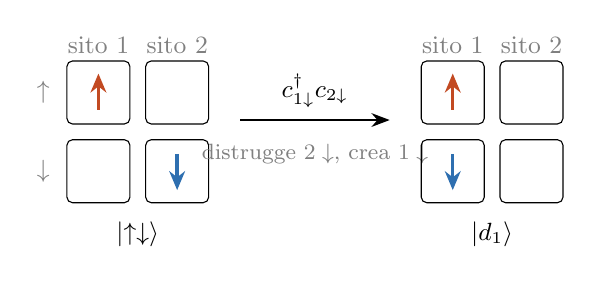
\begin{tikzpicture}[>=Stealth,box/.style={draw,rounded corners=2pt,minimum size=8mm}]
  \node[font=\small,gray] at (0.45,1.2) {sito 1};
  \node[font=\small,gray] at (1.45,1.2) {sito 2};
  \node[font=\small,gray] at (-0.25,0.6) {$\up$};
  \node[font=\small,gray] at (-0.25,-0.4) {$\dn$};
  \node[box] (a11) at (0.45,0.6) {}; \node[box] (a21) at (1.45,0.6) {};
  \node[box] (a12) at (0.45,-0.4) {}; \node[box] (a22) at (1.45,-0.4) {};
  \arrowup{0.45}{0.6}\arrowdn{1.45}{-0.4}
  \node[font=\small] at (0.95,-1.2) {$\ket{\up\dn}$};
  \draw[->,thick] (2.25,0.25) -- (4.15,0.25);
  \node[font=\small] at (3.2,0.62) {$c_{1\dn}^{\dg}c_{2\dn}$};
  \node[font=\footnotesize,gray] at (3.2,-0.18) {distrugge $2\dn$, crea $1\dn$};
  \node[font=\small,gray] at (4.95,1.2) {sito 1};
  \node[font=\small,gray] at (5.95,1.2) {sito 2};
  \node[box] (b11) at (4.95,0.6) {}; \node[box] (b21) at (5.95,0.6) {};
  \node[box] (b12) at (4.95,-0.4) {}; \node[box] (b22) at (5.95,-0.4) {};
  \arrowup{4.95}{0.6}\arrowdn{4.95}{-0.4}
  \node[font=\small] at (5.45,-1.2) {$\ket{d_1}$};
\end{tikzpicture}
\caption{Azione dell'operatore di hopping nei modi (freccia $=$ modo occupato). Da $\ket{\up\dn}$
l'operatore $c_{1\dn}^{\dg}c_{2\dn}$ sposta l'elettrone $\dn$ dal sito 2 al sito 1, producendo la doppia
occupazione $\ket{d_1}$.}
\label{fig:hop}
\end{figure}

\subsection{Costruzione degli stati e azione esplicita di $H_t$}
\label{sub:fermioni}

\paragraph{Base.} A half-filling lo spazio si spezza in due blocchi separati dalla scala $U$:
\begin{align}
\mathcal P\ (E=0):\quad
&\ket{\up\up}=c_{1\up}^{\dg}c_{2\up}^{\dg}\ket{0},\quad
\ket{\up\dn}=c_{1\up}^{\dg}c_{2\dn}^{\dg}\ket{0},\notag\\
&\ket{\dn\up}=c_{1\dn}^{\dg}c_{2\up}^{\dg}\ket{0},\quad
\ket{\dn\dn}=c_{1\dn}^{\dg}c_{2\dn}^{\dg}\ket{0};\\
\mathcal Q\ (E=U):\quad
&\ket{d_1}=c_{1\up}^{\dg}c_{1\dn}^{\dg}\ket{0},\qquad
\ket{d_2}=c_{2\up}^{\dg}c_{2\dn}^{\dg}\ket{0}.
\end{align}

\paragraph{Calcolo di $H_t\ket{\up\dn}$ (tutti i termini).} Con $H_t=-t\big(c_{1\up}^{\dg}c_{2\up}
+c_{1\dn}^{\dg}c_{2\dn}+c_{2\up}^{\dg}c_{1\up}+c_{2\dn}^{\dg}c_{1\dn}\big)$ e
$\ket{\up\dn}=c_{1\up}^{\dg}c_{2\dn}^{\dg}\ket{0}$, due dei quattro termini si annullano subito:
$-t\,c_{1\up}^{\dg}c_{2\up}$ contiene $c_{2\up}$ (sul sito 2 c'è $\dn$, non $\up$) e
$-t\,c_{2\dn}^{\dg}c_{1\dn}$ contiene $c_{1\dn}$ (sul sito 1 c'è $\up$); entrambi danno $0$. Il termine
$-t\,c_{1\dn}^{\dg}c_{2\dn}$ dà invece, portando $c_{2\dn}$ verso destra:
\begin{align}
-t\,c_{1\dn}^{\dg}c_{2\dn}\,c_{1\up}^{\dg}c_{2\dn}^{\dg}\ket{0}
&=-t\,c_{1\dn}^{\dg}\big(-c_{1\up}^{\dg}\,\underbrace{c_{2\dn}c_{2\dn}^{\dg}}_{1-\opn_{2\dn}}\big)\ket{0}
=-t\,c_{1\dn}^{\dg}\big(-c_{1\up}^{\dg}\big)\ket{0}\notag\\
&= t\,c_{1\dn}^{\dg}c_{1\up}^{\dg}\ket{0}
= -t\,c_{1\up}^{\dg}c_{1\dn}^{\dg}\ket{0} = -t\,\ket{d_1},
\end{align}
dove si è usato $\{c_{2\dn},c_{1\up}^{\dg}\}=0$ (segno $-$) e poi $c_{2\dn}c_{2\dn}^{\dg}\ket{0}=\ket{0}$;
l'ultimo passaggio riordina in forma canonica ($c_{1\dn}^{\dg}c_{1\up}^{\dg}=-c_{1\up}^{\dg}c_{1\dn}^{\dg}$).
Analogamente, $-t\,c_{2\up}^{\dg}c_{1\up}$ dà $-t\,\ket{d_2}$: portando $c_{1\up}$ a destra,
$c_{1\up}c_{1\up}^{\dg}c_{2\dn}^{\dg}\ket{0}=(1-\opn_{1\up})c_{2\dn}^{\dg}\ket{0}=c_{2\dn}^{\dg}\ket{0}$,
quindi $-t\,c_{2\up}^{\dg}c_{2\dn}^{\dg}\ket{0}=-t\,\ket{d_2}$.
In totale $H_t\ket{\up\dn}=-t(\ket{d_1}+\ket{d_2})$. Ripetendo identici passaggi:
\begin{equation}
\boxed{\;H_t\ket{\up\dn}=-t\big(\ket{d_1}+\ket{d_2}\big),\quad
H_t\ket{\dn\up}=+t\big(\ket{d_1}+\ket{d_2}\big),\quad
H_t\ket{\up\up}=H_t\ket{\dn\dn}=0.\;}
\label{eq:Htaction}
\end{equation}
Gli stati paralleli si annullano perché spostare un $\up$ su un sito con già un $\up$ darebbe
$c_{i\up}^{\dg}c_{i\up}^{\dg}=0$ (Pauli). Il \emph{segno opposto} fra $\ket{\up\dn}$ e $\ket{\dn\up}$
nasce dal diverso numero di anticommutazioni necessarie a riordinare gli operatori, e sarà la sorgente
del termine fuori diagonale e dell'interferenza (Sezione~\ref{sub:interferenza}).

\subsection{$H_U$ diagonale, $H_t$ fuori dai blocchi, e la matrice $6\times6$}
\label{sub:blocchi}

\paragraph{$H_U$ è diagonale.} Gli $\opn_{i\sigma}$ contano (autovalori $0,1$). Ad esempio
\[
\opn_{1\up}\ket{\up\dn}=c_{1\up}^{\dg}\big(c_{1\up}c_{1\up}^{\dg}\big)c_{2\dn}^{\dg}\ket{0}
=c_{1\up}^{\dg}c_{2\dn}^{\dg}\ket{0}=\ket{\up\dn},\qquad \opn_{1\dn}\ket{\up\dn}=0,
\]
quindi $\opn_{1\up}\opn_{1\dn}\ket{\up\dn}=0$. Su ogni stato di $\mathcal P$ ciascun sito ha un solo
elettrone, dunque $H_U=0$; su $\ket{d_{1,2}}$ un sito è doppiamente occupato e $H_U=U$. Pertanto $H_U$ è
diagonale con autovalori $0$ (su $\mathcal P$) e $U$ (su $\mathcal Q$).

\paragraph{$H_t$ non ha elementi dentro $\mathcal P$.} Da~\eqref{eq:Htaction}, $H_t\ket{\beta}$ atterra
sempre in $\mathcal Q$ (o si annulla): un singolo salto svuota un sito e ne raddoppia un altro. Poiché
$\mathcal P\perp\mathcal Q$, per ogni $\alpha,\beta\in\mathcal P$ si ha
$\melem{\alpha}{H_t}{\beta}=0$. Per tornare da $\mathcal P$ a $\mathcal P$ servono \emph{due} salti.

\paragraph{Costruzione della matrice.} Gli elementi non nulli si leggono direttamente
da~\eqref{eq:Htaction}: $\melem{d_1}{H_t}{\up\dn}=-t$ (coefficiente di $\ket{d_1}$ in $H_t\ket{\up\dn}$),
$\melem{d_2}{H_t}{\up\dn}=-t$, $\melem{d_1}{H_t}{\dn\up}=+t$, $\melem{d_2}{H_t}{\dn\up}=+t$; gli elementi
con righe/colonne $\ket{\up\up},\ket{\dn\dn}$ sono nulli. Aggiungendo $H_U$ (diagonale, $U$ sui due stati
$\mathcal Q$) si ottiene la Figura~\ref{fig:block}.

\begin{figure}[htbp]
\centering
\renewcommand{\arraystretch}{1.25}
\[
\begin{NiceArray}{r|cccccc}[margin]
 & \ket{\up\up} & \ket{\up\dn} & \ket{\dn\up} & \ket{\dn\dn} & \ket{d_1} & \ket{d_2} \\
\hline
\ket{\up\up} & 0 & 0 & 0 & 0 & 0 & 0 \\
\ket{\up\dn} & 0 & 0 & 0 & 0 & -t & -t \\
\ket{\dn\up} & 0 & 0 & 0 & 0 & +t & +t \\
\ket{\dn\dn} & 0 & 0 & 0 & 0 & 0 & 0 \\
\ket{d_1} & 0 & -t & +t & 0 & U & 0 \\
\ket{d_2} & 0 & -t & +t & 0 & 0 & U \\
\CodeAfter
  \begin{tikzpicture}
    \fill[blockP,opacity=0.55] (2-|2) rectangle (6-|6);
    \fill[blockC,opacity=0.6] (2-|6) rectangle (6-|8);
    \fill[blockC,opacity=0.6] (6-|2) rectangle (8-|6);
    \fill[blockQ,opacity=0.7] (6-|6) rectangle (8-|8);
  \end{tikzpicture}
\end{NiceArray}
\]
\caption{La matrice $6\times6$ di $H=H_t+H_U$. Blocco $\mathcal P$--$\mathcal P$ (grigio) nullo; blocco
$\mathcal Q$--$\mathcal Q$ (verde) diagonale $U\mathbb{I}$; blocchi di accoppiamento $\mathcal P$--$\mathcal Q$
(ambra) con le sole entrate $\pm t$ sulle righe/colonne antiparallele.}
\label{fig:block}
\end{figure}

\FloatBarrier
\subsection{Scambio cinetico: salto virtuale, canale, repulsione tra livelli}
\label{sub:cinetico}

\paragraph{Il salto è ``virtuale''.} Nel regime $U\gg t$ lo stato $\ket{d}$ sta a energia $U$, troppo
alta perché il sistema vi finisca davvero conservando l'energia: un salto \emph{reale} richiederebbe di
fornire $U$ dall'esterno. Quello che accade è un processo \emph{virtuale}: il sistema esplora
momentaneamente $\ket{d}$ e torna indietro, consentito dall'indeterminazione tempo--energia (occupazione
per $\Delta t\sim\hbar/U$). Formalmente $\ket{d}$ compare solo come stato \emph{intermedio} nella somma
del secondo ordine, mai come stato finale.

\paragraph{L'``esistenza del canale''.} Il canale è l'elemento di matrice $\melem{d}{H_t}{\up\dn}\neq0$:
la via per cui $H_t$ può connettere lo stato antiparallelo all'intermedio. La sua esistenza fa sì che il
fondamentale non sia $\ket{\up\dn}$ puro ma acquisti una piccola ammixtura di $\ket{d}$ (quantificata sotto).
Per spin paralleli quell'elemento è nullo (Pauli vieta il salto): il canale è chiuso.

\paragraph{Perché abbassa l'energia: una repulsione tra livelli.} Per isolare il meccanismo, consideriamo
il modello a \emph{singolo canale}: un solo stato antiparallelo $\ket{\up\dn}$ (a $E_0=0$) accoppiato a un
solo intermedio $\ket{d}$ (a $E_d=U$) tramite $\melem{d}{H_t}{\up\dn}=t$. La matrice è
\begin{equation}
H_{2\times2}=\begin{pmatrix} 0 & t\\ t & U\end{pmatrix}.
\label{eq:H2x2}
\end{equation}
Gli autovalori si ottengono dall'\textbf{equazione secolare} $\det(H_{2\times2}-E\,\mathbb{I})=0$:
\begin{equation}
\det\begin{pmatrix} -E & t\\ t & U-E\end{pmatrix}=(-E)(U-E)-t^2=E^2-UE-t^2=0
\ \Longrightarrow\
\boxed{\,E_\pm=\frac{U}{2}\pm\sqrt{\Big(\frac{U}{2}\Big)^2+t^2}\,}.
\label{eq:Epm}
\end{equation}
Controlli da Vi\`ete: traccia $E_++E_-=U$ (somma diagonale $0+U$) e determinante $E_+E_-=-t^2$
($=0\cdot U-t\cdot t$). Da $E_+E_-=-t^2<0$ segue che un autovalore è positivo e uno negativo: $E_-<0$
scende sotto lo zero di partenza, $E_+>U$ sale sopra. I livelli si \emph{respingono}
(Figura~\ref{fig:repulsion}).

\paragraph{L'approssimazione $t\ll U$, in dettaglio.} Il parametro piccolo adimensionale è $t/U$. Si
espande la radice con $\sqrt{1+x}=1+\tfrac12 x-\tfrac18 x^2+\dots$ e $x=(2t/U)^2$:
\begin{equation}
\sqrt{\Big(\tfrac{U}{2}\Big)^2+t^2}=\frac{U}{2}\sqrt{1+\Big(\tfrac{2t}{U}\Big)^2}
=\frac{U}{2}\Big[1+2\frac{t^2}{U^2}-2\frac{t^4}{U^4}+\dots\Big]
=\frac{U}{2}+\frac{t^2}{U}-\frac{t^4}{U^3}+\dots
\end{equation}
da cui, separando i due segni,
\begin{equation}
E_-=-\frac{t^2}{U}+\frac{t^4}{U^3}-\dots\ \xrightarrow{t\ll U}\ -\frac{t^2}{U},\qquad
E_+=U+\frac{t^2}{U}-\dots\ \xrightarrow{t\ll U}\ U+\frac{t^2}{U}.
\label{eq:Epm-approx}
\end{equation}
Tre punti da fissare:
\begin{itemize}[nosep]
\item \textbf{Cosa si trattiene/butta.} Il termine guida $-t^2/U$ è \emph{esattamente} il risultato della
teoria perturbativa al secondo ordine in $t$. Il primo termine trascurato è $O(t^4/U^3)$ (quarto ordine);
l'\textbf{errore relativo} sul livello è quindi $\sim(t/U)^2$.
\item \textbf{Quando vale.} Serve $U\gg t$ (regime di Mott): la doppia occupazione è così costosa da essere
solo virtuale. Se $t\sim U$ lo sviluppo collassa, le fluttuazioni di carica non sono trascurabili e la
descrizione di soli spin perde senso.
\item \textbf{Dove sta l'approssimazione.} Non nel diagonalizzare, ma nel \emph{troncare} la serie al
secondo ordine. La $\Heff$ vera (Sezione~\ref{sub:interferenza}) si diagonalizza esattamente: l'approssimazione
è già ``congelata'' dentro al coefficiente $J=4t^2/U$.
\end{itemize}

\paragraph{Angolo di mescolamento e ammixtura.} L'autostato basso esatto non è $\ket{\up\dn}$ puro ma
$\cos\theta\,\ket{\up\dn}+\sin\theta\,\ket{d}$, con angolo dato (per una matrice simmetrica
$2\times2$ $\big(\begin{smallmatrix}\epsilon_1 & v\\ v & \epsilon_2\end{smallmatrix}\big)$) da
$\tan2\theta=\dfrac{2v}{\epsilon_1-\epsilon_2}=\dfrac{2t}{0-U}=-\dfrac{2t}{U}$. Per $t\ll U$,
$\theta\approx-t/U$, cioè $\ket{\psi_-}\approx\ket{\up\dn}-\tfrac{t}{U}\ket{d}$: ammixtura di ampiezza
$\sim t/U$ e probabilità $\sim(t/U)^2$ dello stato virtuale. È piccola proprio nel regime $U\gg t$, ed è
ciò che rende lecito proiettare la dinamica su $\mathcal P$.

\begin{figure}[htbp]
\centering
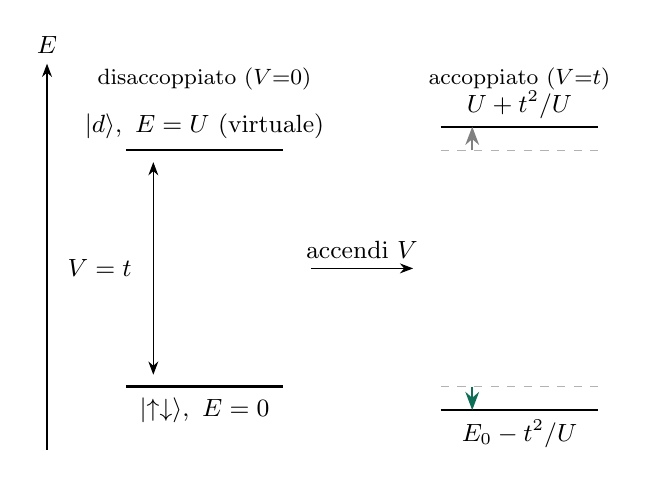
\begin{tikzpicture}[>=Stealth]
  \draw[->] (0,-0.2) -- (0,4.7) node[above,font=\small] {$E$};
  \node[font=\footnotesize] at (2,4.5) {disaccoppiato ($V{=}0$)};
  \node[font=\footnotesize] at (6,4.5) {accoppiato ($V{=}t$)};
  \draw[thick] (1,0.6) -- (3,0.6); \node[font=\small] at (2,0.3) {$\ket{\up\dn},\ E=0$};
  \draw[thick] (1,3.6) -- (3,3.6); \node[font=\small] at (2,3.9) {$\ket{d},\ E=U$ (virtuale)};
  \draw[<->] (1.35,0.75) -- (1.35,3.45); \node[font=\small,anchor=east] at (1.2,2.1) {$V=t$};
  \draw[->] (3.35,2.1) -- (4.65,2.1) node[midway,above,font=\small] {accendi $V$};
  \draw[gray!60,dashed] (5,0.6) -- (7.1,0.6);
  \draw[gray!60,dashed] (5,3.6) -- (7.1,3.6);
  \draw[thick] (5,0.3) -- (7,0.3); \node[font=\small] at (6,0.0) {$E_0-t^2/U$};
  \draw[thick] (5,3.9) -- (7,3.9); \node[font=\small] at (6,4.18) {$U+t^2/U$};
  \draw[teal,->,thick] (5.4,0.6) -- (5.4,0.3);
  \draw[gray,->,thick] (5.4,3.6) -- (5.4,3.9);
\end{tikzpicture}
\caption{Repulsione tra livelli (modello a singolo canale). Accendendo $V=t$ il livello basso
$\ket{\up\dn}$ scende a $-t^2/U$, mentre lo stato virtuale $\ket{d}$ sale a $U+t^2/U$. È quest'ultimo (non
lo stato di $\mathcal P$) a salire.}
\label{fig:repulsion}
\end{figure}

\begin{figure}[htbp]
\centering
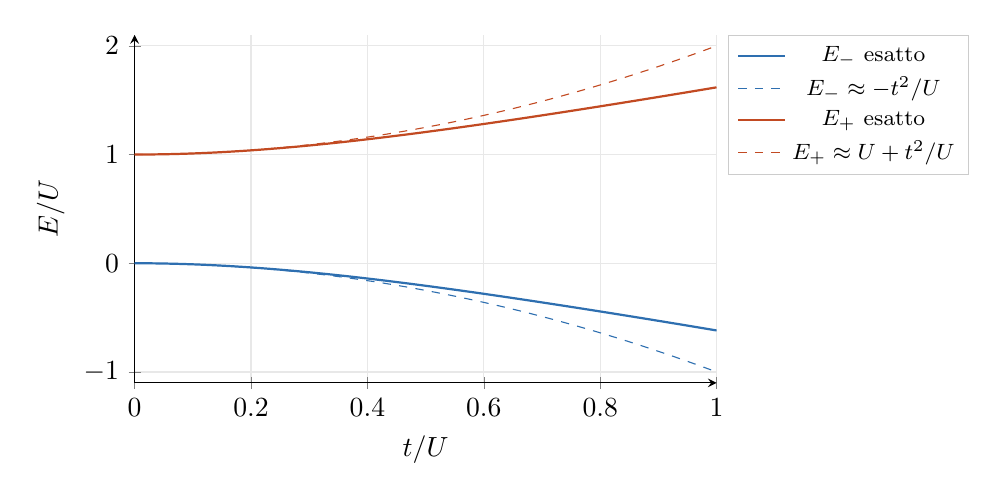
\begin{tikzpicture}
\begin{axis}[
  width=0.74\linewidth, height=6.0cm,
  xlabel={$t/U$}, ylabel={$E/U$},
  xmin=0, xmax=1, ymin=-1.1, ymax=2.1,
  axis lines=left, grid=both, grid style={gray!18},
  legend style={font=\footnotesize, at={(1.02,1)}, anchor=north west, draw=gray!40},
]
\addplot[spindown,thick,domain=0:1,samples=80]{0.5-sqrt(0.25+x^2)}; \addlegendentry{$E_-$ esatto}
\addplot[spindown,dashed,domain=0:1,samples=80]{-x^2};              \addlegendentry{$E_-\approx-t^2/U$}
\addplot[spinup,thick,domain=0:1,samples=80]{0.5+sqrt(0.25+x^2)};   \addlegendentry{$E_+$ esatto}
\addplot[spinup,dashed,domain=0:1,samples=80]{1+x^2};               \addlegendentry{$E_+\approx U+t^2/U$}
\end{axis}
\end{tikzpicture}
\caption{Autovalori esatti~\eqref{eq:Epm} (continui) contro le approssimazioni al secondo
ordine~\eqref{eq:Epm-approx} (tratteggiati), in funzione di $t/U$. Coincidono per $t/U\lesssim0.3$ e si
discostano progressivamente: l'approssimazione $-t^2/U$ sovrastima l'abbassamento perché trascura
$+t^4/U^3$. È la regione $t/U\ll1$ in cui il modello di spin con $J=4t^2/U$ è affidabile.}
\label{fig:exactapprox}
\end{figure}

\FloatBarrier
\subsection{Teoria perturbativa al secondo ordine: la formula e i suoi elementi}
\label{sub:secondorder}

Il modello a singolo canale dà l'intuizione; il calcolo rigoroso tiene conto di \emph{entrambi} gli stati
virtuali $\ket{d_1},\ket{d_2}$ e di \emph{entrambi} gli stati antiparalleli. Poiché $H_t$ non agisce
dentro $\mathcal P$ (il primo ordine si annulla), l'effetto compare al secondo ordine. Per un sottospazio
$\mathcal P$ degenere a energia $E_0$, con perturbazione $V=H_t$ che connette solo $\mathcal P\to\mathcal Q$,
la teoria perturbativa degenere (trasformazione di Schrieffer--Wolff) dà l'\textbf{Hamiltoniana efficace}
\begin{equation}
(\Heff)_{\alpha\beta}=\sum_{m\in\mathcal Q}\frac{\melem{\alpha}{H_t}{m}\melem{m}{H_t}{\beta}}{E_0-E_m}
=-\frac1U\sum_{m\in\mathcal Q}\melem{\alpha}{H_t}{m}\melem{m}{H_t}{\beta},
\qquad \alpha,\beta\in\mathcal P,
\label{eq:secondorder}
\end{equation}
con $E_0=0$, $E_m=U$ e denominatore $E_0-E_m=-U$ (Figura~\ref{fig:super}). Ogni termine si legge come un
cammino a due salti: ampiezza d'ingresso $\times$ propagatore $(-1/U)$ $\times$ ampiezza d'uscita.

\begin{figure}[htbp]
\centering
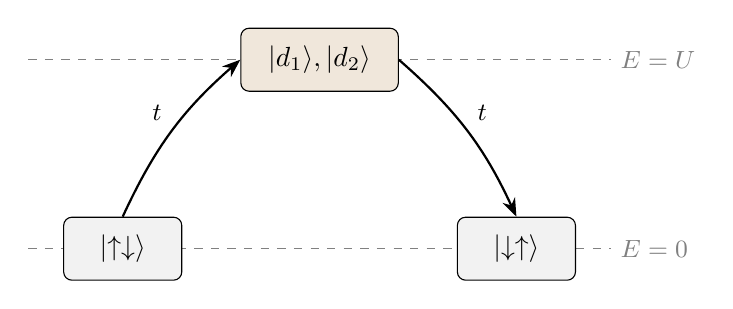
\begin{tikzpicture}[>=Stealth,st/.style={draw,rounded corners=3pt,minimum width=1.5cm,minimum height=0.8cm}]
  \draw[dashed,gray] (-0.2,0) -- (7.2,0); \node[gray,font=\small,anchor=west] at (7.2,0) {$E=0$};
  \draw[dashed,gray] (-0.2,2.4) -- (7.2,2.4); \node[gray,font=\small,anchor=west] at (7.2,2.4) {$E=U$};
  \node[st,fill=gray!10] (l) at (1,0) {$\ket{\up\dn}$};
  \node[st,fill=gray!10] (r) at (6,0) {$\ket{\dn\up}$};
  \node[st,fill=amber!15,minimum width=2cm] (d) at (3.5,2.4) {$\ket{d_1},\ket{d_2}$};
  \draw[->,thick] (l.north) to[bend left=12] node[above left,font=\small] {$t$} (d.west);
  \draw[->,thick] (d.east) to[bend left=12] node[above right,font=\small] {$t$} (r.north);
\end{tikzpicture}
\caption{Processo di superscambio al secondo ordine: due salti $t$ collegano $\ket{\up\dn}$ allo stato
virtuale (a energia $U$) e poi a $\ket{\dn\up}$, con propagatore $1/(0-U)=-1/U$.}
\label{fig:super}
\end{figure}

\paragraph{Elementi di matrice, espliciti.} Servono i coefficienti, letti da~\eqref{eq:Htaction}:
$\melem{d_{1,2}}{H_t}{\up\dn}=-t$ e $\melem{d_{1,2}}{H_t}{\dn\up}=+t$ (e i bra coniugati uguali, essendo
reali). Allora, dalla~\eqref{eq:secondorder},
\begin{align}
(\Heff)_{\up\dn,\,\up\dn}
&=-\frac1U\sum_{m=d_1,d_2}\melem{\up\dn}{H_t}{m}\melem{m}{H_t}{\up\dn}
=-\frac1U\big[(-t)(-t)+(-t)(-t)\big]=-\frac{2t^2}{U},\\
(\Heff)_{\dn\up,\,\up\dn}
&=-\frac1U\sum_{m=d_1,d_2}\melem{\dn\up}{H_t}{m}\melem{m}{H_t}{\up\dn}
=-\frac1U\big[(+t)(-t)+(+t)(-t)\big]=+\frac{2t^2}{U},
\end{align}
e analogamente $(\Heff)_{\dn\up,\dn\up}=-\tfrac{2t^2}{U}$, $(\Heff)_{\up\dn,\dn\up}=+\tfrac{2t^2}{U}$; tutti
gli elementi con stati paralleli sono nulli. I due tipi di percorso sono in Figura~\ref{fig:twohop}: il
\emph{ritorno} (diagonale, $-t^2/U$ per ciascun $\ket{d}$) e lo \emph{scambio} (fuori diagonale, $+t^2/U$).

\begin{figure}[htbp]
\centering
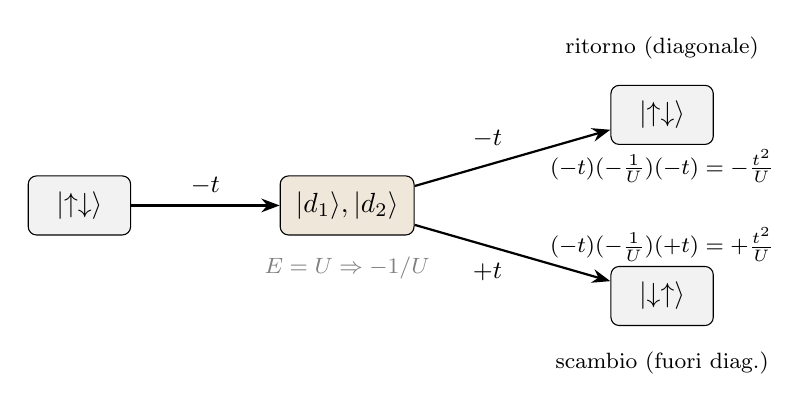
\begin{tikzpicture}[>=Stealth,st/.style={draw,rounded corners=3pt,minimum width=1.3cm,minimum height=0.75cm}]
  \node[st,fill=gray!10] (s) at (0,0) {$\ket{\up\dn}$};
  \node[st,fill=amber!15,minimum width=1.7cm] (d) at (3.4,0) {$\ket{d_1},\ket{d_2}$};
  \node[font=\footnotesize,gray] at (3.4,-0.8) {$E=U\Rightarrow -1/U$};
  \node[st,fill=gray!10] (rt) at (7.4,1.15) {$\ket{\up\dn}$};
  \node[st,fill=gray!10] (rb) at (7.4,-1.15) {$\ket{\dn\up}$};
  \draw[->,thick] (s) -- node[above,font=\small]{$-t$} (d);
  \draw[->,thick] (d) -- node[above left,font=\small]{$-t$} (rt);
  \draw[->,thick] (d) -- node[below left,font=\small]{$+t$} (rb);
  \node[font=\footnotesize] at (7.4,2.0) {ritorno (diagonale)};
  \node[font=\footnotesize] at (7.4,0.5) {$(-t)(-\tfrac1U)(-t)=-\tfrac{t^2}{U}$};
  \node[font=\footnotesize] at (7.4,-0.5) {$(-t)(-\tfrac1U)(+t)=+\tfrac{t^2}{U}$};
  \node[font=\footnotesize] at (7.4,-2.0) {scambio (fuori diag.)};
\end{tikzpicture}
\caption{Percorsi al secondo ordine da $\ket{\up\dn}$: il ``ritorno'' dà $-t^2/U$, lo ``scambio''
$+t^2/U$ (per ciascuno dei due stati virtuali). Il segno opposto è la chiave dell'interferenza.}
\label{fig:twohop}
\end{figure}

\FloatBarrier
\subsection{Dagli elementi di matrice alle energie: diagonalizzazione e interferenza}
\label{sub:interferenza}

\emph{Punto delicato.} ``Ritorno'' e ``scambio'' \textbf{non} sono due destini energetici dei due stati
antiparalleli: sono gli elementi \emph{diagonale} e \emph{fuori diagonale} di $\Heff$. L'elemento fuori
diagonale \emph{accoppia} $\ket{\up\dn}$ e $\ket{\dn\up}$, perciò $\ket{\up\dn}$ da solo \textbf{non è un
autostato} e non ha un'energia definita. Le energie si ottengono solo \textbf{diagonalizzando}
\begin{equation}
\Heff\big|_{\{\ket{\up\dn},\ket{\dn\up}\}}
=\begin{pmatrix} -\frac{2t^2}{U} & +\frac{2t^2}{U}\\[3pt] +\frac{2t^2}{U} & -\frac{2t^2}{U}\end{pmatrix}
\equiv\begin{pmatrix} a & b\\ b & a\end{pmatrix},\qquad a=-\tfrac{2t^2}{U},\ b=+\tfrac{2t^2}{U}.
\end{equation}
L'equazione secolare $\det\big(\begin{smallmatrix} a-E & b\\ b & a-E\end{smallmatrix}\big)=(a-E)^2-b^2=0$ dà
$E=a\pm b$:
\begin{equation}
\text{singoletto (antisim.)}:\ E=a-b=-\frac{4t^2}{U},\qquad
\text{tripletto }T_0\text{ (sim.)}:\ E=a+b=0 .
\label{eq:autovalori}
\end{equation}
La diagonale abbassa entrambi gli antiparalleli di $2t^2/U$; la fuori diagonale li \emph{separa} di
$\pm2t^2/U$, portando il singoletto a $-4t^2/U$ e riportando il tripletto a $0$ (Figura~\ref{fig:constr}).
Non esiste alcun livello a $E_0+t^2/U$.

\begin{figure}[htbp]
\centering
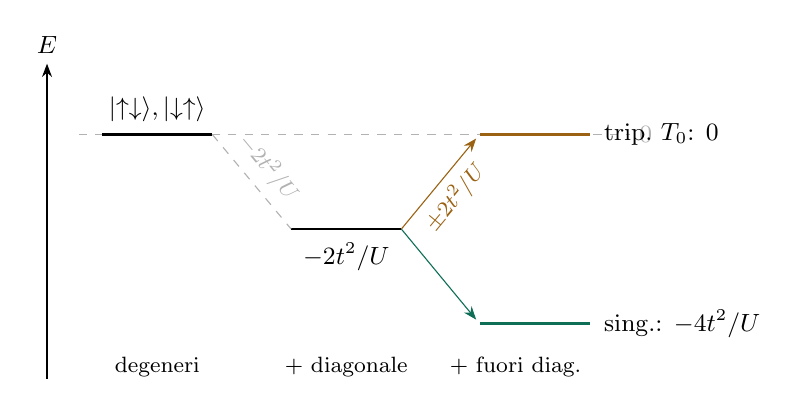
\begin{tikzpicture}[>=Stealth]
  \draw[->] (0,-3.1) -- (0,0.9) node[above,font=\small] {$E$};
  \draw[gray!60,dashed] (0.4,0) -- (7.4,0) node[right,font=\small] {$0$};
  \draw[thick] (0.7,0) -- (2.1,0); \node[font=\small] at (1.4,0.32) {$\ket{\up\dn},\ket{\dn\up}$};
  \node[font=\footnotesize] at (1.4,-2.95) {degeneri};
  \draw[thick] (3.1,-1.2) -- (4.5,-1.2); \node[font=\small] at (3.8,-1.55) {$-2t^2/U$};
  \node[font=\footnotesize] at (3.8,-2.95) {$+$ diagonale};
  \draw[amber,thick] (5.5,0) -- (6.9,0); \node[font=\small,anchor=west] at (6.95,0) {trip.\ $T_0$: $0$};
  \draw[teal,thick] (5.5,-2.4) -- (6.9,-2.4); \node[font=\small,anchor=west] at (6.95,-2.4) {sing.: $-4t^2/U$};
  \node[font=\footnotesize] at (5.95,-2.95) {$+$ fuori diag.};
  \draw[gray!60,dashed] (2.1,0) -- (3.1,-1.2) node[midway,above,font=\footnotesize,sloped] {$-2t^2/U$};
  \draw[teal,->] (4.5,-1.2) -- (5.45,-2.35);
  \draw[amber,->] (4.5,-1.2) -- (5.45,-0.05) node[midway,below,font=\footnotesize,sloped] {$\pm2t^2/U$};
\end{tikzpicture}
\caption{Costruzione degli autovalori di $\Heff$. Gli antiparalleli, degeneri a $E=0$, vengono abbassati
dalla diagonale a $-2t^2/U$ e poi separati dalla fuori diagonale: singoletto a $-4t^2/U$, tripletto $T_0$
di nuovo a $0$.}
\label{fig:constr}
\end{figure}

\paragraph{Interferenza tra i due percorsi.} Lo stesso risultato, letto come interferenza, è più
trasparente. Da $\Heff\ket{\up\dn}=-\tfrac{2t^2}{U}\ket{\up\dn}+\tfrac{2t^2}{U}\ket{\dn\up}$ (e simmetrico
per $\ket{\dn\up}$), e usando $\ket{S}=\tfrac1{\sqrt2}(\ket{\up\dn}-\ket{\dn\up})$,
$\ket{T_0}=\tfrac1{\sqrt2}(\ket{\up\dn}+\ket{\dn\up})$:
\begin{align}
\Heff\ket{S}
&=\tfrac1{\sqrt2}\Big[\big(-\tfrac{2t^2}{U}\ket{\up\dn}+\tfrac{2t^2}{U}\ket{\dn\up}\big)
-\big(-\tfrac{2t^2}{U}\ket{\dn\up}+\tfrac{2t^2}{U}\ket{\up\dn}\big)\Big]\notag\\
&=\tfrac1{\sqrt2}\Big[-\tfrac{4t^2}{U}\ket{\up\dn}+\tfrac{4t^2}{U}\ket{\dn\up}\Big]=-\frac{4t^2}{U}\ket{S},
\label{eq:interfS}\\[2pt]
\Heff\ket{T_0}
&=\tfrac1{\sqrt2}\Big[\big(-\tfrac{2t^2}{U}\ket{\up\dn}+\tfrac{2t^2}{U}\ket{\dn\up}\big)
+\big(-\tfrac{2t^2}{U}\ket{\dn\up}+\tfrac{2t^2}{U}\ket{\up\dn}\big)\Big]=0 . \label{eq:interfT}
\end{align}
Per il singoletto i due contributi (ritorno e scambio) \textbf{si sommano} (interferenza costruttiva,
abbassamento massimo); per il tripletto \textbf{si cancellano} (interferenza distruttiva). È il segno
relativo $-$/$+$ della sovrapposizione a decidere il segno dell'interferenza, e quindi a selezionare il
singoletto come fondamentale.

\paragraph{Due diagonalizzazioni da non confondere.} Il $+t^2/U$ che \emph{alza} un livello appartiene
all'accoppiamento $\mathcal P$--$\mathcal Q$ \eqref{eq:Epm-approx} e riguarda lo stato virtuale $\ket{d}$,
non lo stato antiparallelo di $\mathcal P$:
\begin{center}
\begin{tabular}{lll}
\toprule
accoppiamento & stati coinvolti & risultato \\
\midrule
$\mathcal P$--$\mathcal Q$ & $\ket{\up\dn}\leftrightarrow\ket{d}$ & basso $\to -t^2/U$;\quad $\ket{d}\to U+t^2/U$ \\
$\mathcal P$--$\mathcal P$ (effettivo) & $\ket{\up\dn}\leftrightarrow\ket{\dn\up}$ & singoletto $\to -4t^2/U$;\quad tripletto $\to 0$ \\
\bottomrule
\end{tabular}
\end{center}

\FloatBarrier
\subsection{L'Hamiltoniana efficace e la mappa sugli spin: $J=4t^2/U$}
\label{sub:efficace}

\begin{nota}[Che cosa significa $\Heff$]
$\Heff$ sta per \textbf{Hamiltoniana efficace} (\emph{effective Hamiltonian}): è l'operatore che descrive
la fisica di bassa energia agendo \emph{solo} sul sottospazio $\mathcal P$, dopo aver eliminato gli stati
di $\mathcal Q$. L'Hamiltoniana ``vera''~\eqref{eq:hubbard} agisce su 6 stati; a $U\gg t$ gli stati di
$\mathcal Q$ sono inaccessibili come stati reali e si riassorbono perturbativamente in un operatore più
piccolo, definito sui 4 stati di $\mathcal P$, i cui autovalori riproducono -- all'ordine $t^2/U$ -- i
livelli bassi. È quindi \emph{approssimata} (vale tanto meglio quanto più $U/t$ è grande) e \emph{non
agisce sullo stesso spazio} dell'originale: è una descrizione ridotta.
\end{nota}

\paragraph{Operatori di spin in seconda quantizzazione.} Lo spin dell'elettrone sul sito $i$ è
$\sv_i=\tfrac12\sum_{\sigma\sigma'}c_{i\sigma}^{\dg}\boldsymbol{\sigma}_{\sigma\sigma'}c_{i\sigma'}$, ovvero
\begin{equation}
s_i^z=\tfrac12(\opn_{i\up}-\opn_{i\dn}),\qquad s_i^+=c_{i\up}^{\dg}c_{i\dn},\qquad s_i^-=c_{i\dn}^{\dg}c_{i\up}.
\end{equation}
Nel sottospazio a singola occupazione questi agiscono come normali operatori di spin-$\tfrac12$
(Appendice~\ref{app:spin}). Il prodotto scalare si decompone come
\begin{equation}
\sv_1\!\cdot\sv_2=s_1^xs_2^x+s_1^ys_2^y+s_1^zs_2^z=s_1^zs_2^z+\tfrac12\big(s_1^+s_2^-+s_1^-s_2^+\big),
\label{eq:s1s2decomp}
\end{equation}
dove l'ultima uguaglianza segue da $s^x=\tfrac12(s^++s^-)$, $s^y=\tfrac1{2i}(s^+-s^-)$, che danno
$s_1^xs_2^x+s_1^ys_2^y=\tfrac12(s_1^+s_2^-+s_1^-s_2^+)$ (i termini $s^+s^+$ e $s^-s^-$ si cancellano).

\paragraph{$\sv_1\!\cdot\sv_2$ nel settore antiparallelo.} Applicando~\eqref{eq:s1s2decomp} a $\ket{\up\dn}$:
la parte $s_1^zs_2^z$ dà $(+\tfrac12)(-\tfrac12)=-\tfrac14$; la parte flip-flop dà
$\tfrac12 s_1^-s_2^+\ket{\up\dn}=\tfrac12\ket{\dn\up}$ (l'altro termine si annulla). Quindi
\begin{equation}
\sv_1\!\cdot\sv_2\ket{\up\dn}=-\tfrac14\ket{\up\dn}+\tfrac12\ket{\dn\up},\qquad
\sv_1\!\cdot\sv_2\big|_{\{\ket{\up\dn},\ket{\dn\up}\}}=\begin{pmatrix}-\tfrac14 & \tfrac12\\[2pt] \tfrac12 & -\tfrac14\end{pmatrix}.
\end{equation}

\paragraph{Matching che fissa $J$.} Cerchiamo $\Heff=J\big(\sv_1\!\cdot\sv_2-\tfrac14\big)$. Nel settore
antiparallelo,
\[
J\Big(\sv_1\!\cdot\sv_2-\tfrac14\mathbb{I}\Big)
=J\begin{pmatrix}-\tfrac12 & \tfrac12\\[2pt] \tfrac12 & -\tfrac12\end{pmatrix}
=\frac{J}{2}\begin{pmatrix}-1 & 1\\ 1 & -1\end{pmatrix}.
\]
Confrontando con la matrice di $\Heff$ trovata sopra ($-\tfrac{2t^2}{U}$ sulla diagonale): $\tfrac{J}{2}=\tfrac{2t^2}{U}$,
cioè
\begin{equation}
\boxed{\,\Heff=J\Big(\sv_1\!\cdot\sv_2-\tfrac14\Big),\qquad J=\frac{4t^2}{U}>0\,}
\label{eq:Heff}
\end{equation}
(la costante $-\tfrac14$ è uno shift globale e si scarta). Verifica incrociata: sui paralleli
$\sv_1\!\cdot\sv_2=+\tfrac14$ (Appendice~\ref{app:spin}), quindi $J(\tfrac14-\tfrac14)=0$, coerente con
l'assenza di percorsi.

\subsection{Passaggio agli operatori di Pauli}

Con $\sv_i=\tfrac12\boldsymbol{\sigma}_i=\tfrac12(X_i,Y_i,Z_i)$ si ha
$\sv_1\!\cdot\sv_2=\tfrac14\boldsymbol{\sigma}_1\!\cdot\boldsymbol{\sigma}_2=\tfrac14(X_1X_2+Y_1Y_2+Z_1Z_2)$,
quindi
\begin{equation}
\boxed{\,H_{\mathrm{ex}}=J\,\sv_1\!\cdot\sv_2=\frac{J}{4}\big(X_1X_2+Y_1Y_2+Z_1Z_2\big)\,}
\label{eq:Hex}
\end{equation}
che è la forma in operatori da cui parte il documento di riferimento.

\subsection{Perché ``in assenza di accoppiamento spin--orbita''}

Il risultato dipende solo dallo scalare $\sv_1\!\cdot\sv_2$, invariante per rotazioni nello spazio di
spin, perché $t$ e $U$ agiscono sulla carica e lo spin entra solo via Pauli (anch'esso isotropo). Lo
spin--orbita romperebbe questo disaccoppiamento, introducendo termini anisotropi: scambio anisotropo
($J_x\neq J_y\neq J_z$) e il termine antisimmetrico di Dzyaloshinskii--Moriya
$\vec{D}\cdot(\sv_1\times\sv_2)$. Lo trascuriamo perché negli ioni $3d$ leggeri il momento orbitale è in
gran parte ``quenched'' dal campo dei leganti. Il modello isotropo è dunque la descrizione di ordine zero;
l'eventuale termine DM è la perturbazione controllata che rompe le simmetrie.

\FloatBarrier
% =====================================================================
\section{L'Hamiltoniana del dimero e il suo spettro}
\label{sec:dimero}

\subsection{La forma completa}

Aggiungendo all'interazione di scambio l'accoppiamento con un campo magnetico esterno lungo $z$ si ottiene
l'Hamiltoniana~\eqref{eq:Hfull},
\[
H = J\,(X_1X_2+Y_1Y_2+Z_1Z_2) + b\,(Z_1+Z_2),
\]
nel caso isotropo. Il primo termine è l'energia di scambio appena derivata; il secondo è il termine di
\textbf{Zeeman}. (Per coerenza con l'esempio originale, da qui $J$ denota il coefficiente di
$X_1X_2+Y_1Y_2+Z_1Z_2$: a meno di un fattore numerico di convenzione coincide con quello precedente, cfr.\
Appendice~\ref{app:conv}.)

\subsection{Il termine di scambio e il meccanismo di flip-flop}

La parte $Z_1Z_2$ è diagonale ($+1$ sui paralleli, $-1$ sugli antiparalleli). La parte trasversale
$X_1X_2+Y_1Y_2$ è il termine di \textbf{flip-flop}. Con $s_i^{\pm}=\tfrac12(X_i\pm iY_i)$ si ha
$X_i=s_i^++s_i^-$, $Y_i=-i(s_i^+-s_i^-)$, da cui
\begin{equation}
X_1X_2+Y_1Y_2=2\big(s_1^{+}s_2^{-}+s_1^{-}s_2^{+}\big),
\end{equation}
che abbassa uno spin e ne alza un altro, scambiando le configurazioni antiparallele
(Figura~\ref{fig:flipflop}): $(X_1X_2+Y_1Y_2)\ket{\up\dn}=2\ket{\dn\up}$, $(X_1X_2+Y_1Y_2)\ket{\up\up}=0$.
È il termine che mescola $\ket{\up\dn}$ e $\ket{\dn\up}$ e rende il fondamentale entangled.

\begin{figure}[htbp]
\centering
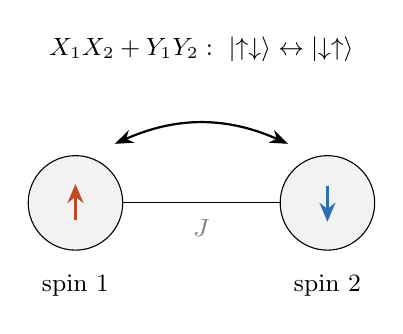
\begin{tikzpicture}[>=Stealth]
  \node[font=\small] at (0,1.95) {$X_1X_2+Y_1Y_2:\ \ket{\up\dn}\leftrightarrow\ket{\dn\up}$};
  \draw[<->,thick] (-1.1,0.75) to[bend left=24] (1.1,0.75);
  \node[circle,draw,fill=gray!10,minimum size=1.2cm] (a) at (-1.6,0) {};
  \node[circle,draw,fill=gray!10,minimum size=1.2cm] (b) at (1.6,0) {};
  \draw (a)--(b); \node[font=\small,gray] at (0,-0.32) {$J$};
  \arrowup{-1.6}{0}\arrowdn{1.6}{0}
  \node[font=\small] at (-1.6,-1.05) {spin 1};
  \node[font=\small] at (1.6,-1.05) {spin 2};
\end{tikzpicture}
\caption{Il termine di flip-flop scambia i due spin quando sono antiparalleli (è nullo sui paralleli, già
autostati). È l'origine microscopica della sovrapposizione singoletto/tripletto.}
\label{fig:flipflop}
\end{figure}

\subsection{Il valore di $\sv_1\!\cdot\sv_2$ su singoletto e tripletto}
\label{sub:s1s2}

\paragraph{Metodo via $S^2$.} Da $S^2=(\sv_1+\sv_2)^2=s_1^2+s_2^2+2\,\sv_1\!\cdot\sv_2$ segue
$\sv_1\!\cdot\sv_2=\tfrac12(S^2-s_1^2-s_2^2)$. Con $s_i^2=s_i(s_i+1)=\tfrac34$ (quindi $s_1^2+s_2^2=\tfrac32$)
e $S^2\to S(S+1)$:
\begin{equation}
\text{singoletto }(S=0):\ \sv_1\!\cdot\sv_2=\tfrac12(0-\tfrac32)=-\tfrac34,\qquad
\text{tripletto }(S=1):\ \sv_1\!\cdot\sv_2=\tfrac12(2-\tfrac32)=+\tfrac14 .
\end{equation}

\paragraph{Metodo diretto.} Da $\sv_1\!\cdot\sv_2\ket{\up\dn}=-\tfrac14\ket{\up\dn}+\tfrac12\ket{\dn\up}$
(e l'analogo per $\ket{\dn\up}$), combinando con i segni della sovrapposizione:
\begin{align}
\sv_1\!\cdot\sv_2\ket{S}
&=\tfrac1{\sqrt2}\Big[\big(-\tfrac14\ket{\up\dn}+\tfrac12\ket{\dn\up}\big)-\big(-\tfrac14\ket{\dn\up}+\tfrac12\ket{\up\dn}\big)\Big]
=-\tfrac34\ket{S},\\
\sv_1\!\cdot\sv_2\ket{T_0}
&=\tfrac1{\sqrt2}\Big[\big(-\tfrac14\ket{\up\dn}+\tfrac12\ket{\dn\up}\big)+\big(-\tfrac14\ket{\dn\up}+\tfrac12\ket{\up\dn}\big)\Big]
=+\tfrac14\ket{T_0},
\end{align}
mentre sui paralleli il flip-flop è nullo e resta $s_1^zs_2^z=+\tfrac14$. Di nuovo si vede l'interferenza:
il termine Ising $(-\tfrac14)$ e il flip-flop $(\pm\tfrac12)$ si sommano ($-\tfrac34$, singoletto) o si
cancellano in parte ($+\tfrac14$, tripletto). Le quattro situazioni sono in Figura~\ref{fig:st}.

\begin{figure}[htbp]
\centering
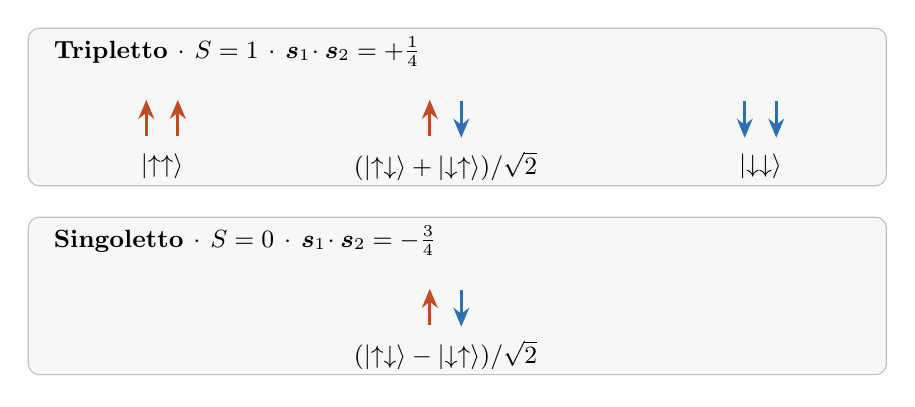
\begin{tikzpicture}[>=Stealth]
  \draw[rounded corners=4pt,fill=gray!6,draw=gray!50] (-0.2,1.0) rectangle (10.7,3.0);
  \node[anchor=west,font=\small\bfseries] at (0.0,2.7) {Tripletto $\cdot$ $S=1$ $\cdot$ $\sv_1\!\cdot\sv_2=+\tfrac14$};
  \arrowup{1.3}{1.85}\arrowup{1.7}{1.85}
  \node[font=\small] at (1.5,1.25) {$\ket{\up\up}$};
  \arrowup{4.9}{1.85}\arrowdn{5.3}{1.85}
  \node[font=\small] at (5.1,1.25) {$(\ket{\up\dn}+\ket{\dn\up})/\sqrt2$};
  \arrowdn{8.9}{1.85}\arrowdn{9.3}{1.85}
  \node[font=\small] at (9.1,1.25) {$\ket{\dn\dn}$};
  \draw[rounded corners=4pt,fill=gray!6,draw=gray!50] (-0.2,-1.4) rectangle (10.7,0.6);
  \node[anchor=west,font=\small\bfseries] at (0.0,0.3) {Singoletto $\cdot$ $S=0$ $\cdot$ $\sv_1\!\cdot\sv_2=-\tfrac34$};
  \arrowup{4.9}{-0.55}\arrowdn{5.3}{-0.55}
  \node[font=\small] at (5.1,-1.15) {$(\ket{\up\dn}-\ket{\dn\up})/\sqrt2$};
\end{tikzpicture}
\caption{Singoletto e tripletto con i rispettivi valori di $\sv_1\!\cdot\sv_2$. Lo stato simmetrico del
tripletto e il singoletto hanno frecce identiche: a distinguerli è solo il segno della sovrapposizione,
che ribalta il valore da $+\tfrac14$ a $-\tfrac34$.}
\label{fig:st}
\end{figure}

\FloatBarrier
\subsection{Spettro analitico}
\label{sub:spettro}

Scriviamo $H=H_1+H_2$. Per il termine di scambio, usando $X_1X_2+Y_1Y_2+Z_1Z_2=4\,\sv_1\!\cdot\sv_2=2(S^2-s_1^2-s_2^2)$,
\begin{equation}
H_1=J(X_1X_2+Y_1Y_2+Z_1Z_2)=2J(S^2-s_1^2-s_2^2)\ \Rightarrow\ H_1\ket{S,M}=2J\big[S(S+1)-\tfrac32\big]\ket{S,M}.
\end{equation}
Per il termine di Zeeman, poiché $S_z=\tfrac12(Z_1+Z_2)$,
\begin{equation}
H_2=b(Z_1+Z_2)=2b\,S_z\ \Rightarrow\ H_2\ket{S,M}=2bM\,\ket{S,M}.
\end{equation}
I due commutano ($H_1\propto S^2$, $H_2\propto S_z$, e $[S^2,S_z]=0$), quindi sono simultaneamente
diagonali in $\ket{S,M}$ e
\begin{equation}
\boxed{\,E(S,M)=2J\,S(S+1)-3J+2bM\,}.
\end{equation}
I quattro livelli sono in Tabella~\ref{tab:livelli}.

\begin{table}[htbp]
\centering
\begin{tabular}{lcccl}
\toprule
stato & $S$ & $M$ & $E$ & (calcolo)\\
\midrule
singoletto & $0$ & $0$ & $-3J$ & $0-3J+0$\\
tripletto & $1$ & $+1$ & $J+2b$ & $4J-3J+2b$\\
tripletto & $1$ & $0$ & $J$ & $4J-3J+0$\\
tripletto & $1$ & $-1$ & $J-2b$ & $4J-3J-2b$\\
\bottomrule
\end{tabular}
\caption{Spettro del dimero isotropo con campo. A campo nullo: singoletto a $-3J$, tripletto degenere a
$+J$, separati da $4J$.}
\label{tab:livelli}
\end{table}

\subsection{Diagramma dei livelli al variare del campo}

Il campo separa linearmente il tripletto in $M$. Lo stato $M=-1$ ($\ket{\dn\dn}$) scende e incrocia il
singoletto: imponendo l'uguaglianza delle energie $-3J=J-2b$ si trova $2b=4J$, cioè $b/J=2$. Sotto soglia
il fondamentale è il singoletto, sopra diventa $\ket{\dn\dn}$ (Figura~\ref{fig:spettro}; qui $B\equiv b$).

\begin{figure}[htbp]
\centering
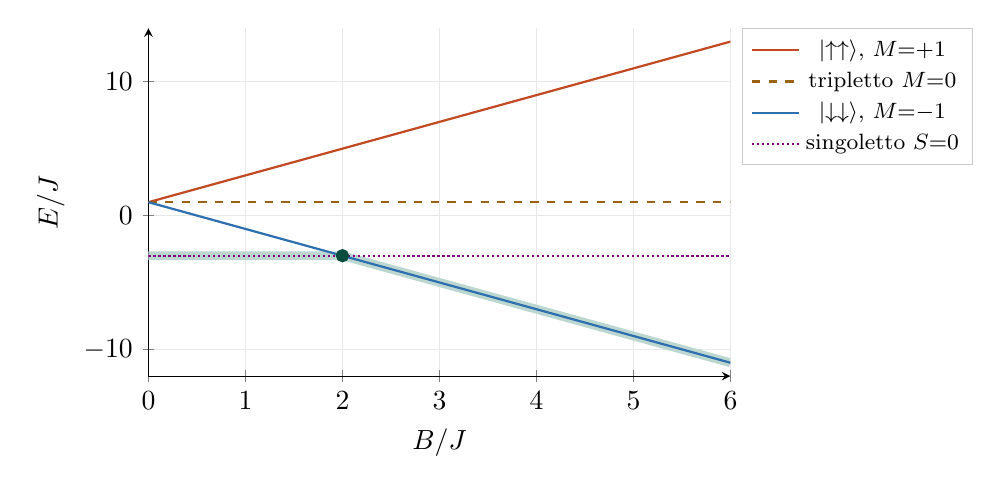
\begin{tikzpicture}
\begin{axis}[
  width=0.74\linewidth, height=6.0cm,
  xlabel={$B/J$}, ylabel={$E/J$},
  xmin=0, xmax=6, ymin=-12, ymax=14,
  domain=0:6, samples=2,
  axis lines=left, grid=both, grid style={gray!18},
  legend style={font=\footnotesize, at={(1.02,1)}, anchor=north west, draw=gray!40},
  every axis plot/.append style={thick},
]
\addplot[line width=3.2pt, teal!28, forget plot] coordinates {(0,-3) (2,-3) (6,-11)};
\addplot[spinup]      {1+2*x}; \addlegendentry{$\ket{\up\up}$, $M{=}{+}1$}
\addplot[amber,dashed]{1};     \addlegendentry{tripletto $M{=}0$}
\addplot[spindown]    {1-2*x}; \addlegendentry{$\ket{\dn\dn}$, $M{=}{-}1$}
\addplot[violet,densely dotted]{-3}; \addlegendentry{singoletto $S{=}0$}
\addplot[only marks, mark=*, mark size=2pt, teal!70!black, forget plot] coordinates {(2,-3)};
\end{axis}
\end{tikzpicture}
\caption{Spettro $E/J$ in funzione di $B/J$. Il singoletto (puntinato) resta a $-3$; il tripletto si
separa: $M{=}{+}1$ sale, $M{=}0$ resta piatto, $M{=}{-}1$ scende. Il fondamentale (banda verde) è il
singoletto fino a $B/J=2$ (punto verde), poi lo stato $M{=}{-}1$.}
\label{fig:spettro}
\end{figure}

\subsection{Osservabili e fidelity}

Sul fondamentale ottenuto via VQE si calcolano osservabili, ad esempio la magnetizzazione
$M_z=(Z_1+Z_2)/2$, il cui valore di aspettazione passa da $0$ (singoletto) a $-1$ (stato $\ket{\dn\dn}$)
attraversando $B/J=2$. La qualità della soluzione variazionale rispetto a quella esatta $\ket{\psi_0}$ si
misura con la fidelity $\mathcal F=\big|\braket{\psi_0}{\psi(\{\tilde\theta_k\})}\big|$.

\FloatBarrier
% =====================================================================
\appendix
\section{Richiamo: algebra di spin-$\tfrac12$}
\label{app:spin}

\paragraph{Matrici di Pauli e operatori di spin.} Con base $\ket{\up}=\binom{1}{0}$, $\ket{\dn}=\binom{0}{1}$,
\[
X=\begin{pmatrix}0&1\\1&0\end{pmatrix},\quad Y=\begin{pmatrix}0&-i\\i&0\end{pmatrix},\quad
Z=\begin{pmatrix}1&0\\0&-1\end{pmatrix},\qquad \sv=\tfrac12(X,Y,Z).
\]
Quindi $s^z\ket{\up}=+\tfrac12\ket{\up}$, $s^z\ket{\dn}=-\tfrac12\ket{\dn}$. Gli operatori a scaletta
$s^{\pm}=s^x\pm is^y=\tfrac12(X\pm iY)$ soddisfano $s^+\ket{\dn}=\ket{\up}$, $s^-\ket{\up}=\ket{\dn}$,
$s^+\ket{\up}=s^-\ket{\dn}=0$, e $s^2=s(s+1)=\tfrac34$.

\paragraph{Stati di spin totale.} Per due spin-$\tfrac12$, $\sv_1+\sv_2=\vec S$ con $S=0$ (singoletto) o
$S=1$ (tripletto):
\[
\ket{S{=}0}=\tfrac1{\sqrt2}(\ket{\up\dn}-\ket{\dn\up}),\qquad
\ket{S{=}1,M}=\Big\{\ket{\up\up},\ \tfrac1{\sqrt2}(\ket{\up\dn}+\ket{\dn\up}),\ \ket{\dn\dn}\Big\}.
\]
Sono autostati di $S^2$ con autovalore $S(S+1)$ e di $S_z$ con autovalore $M$.

\paragraph{Identità utili.} $\boldsymbol{\sigma}_1\!\cdot\boldsymbol{\sigma}_2=2\,\mathrm{SWAP}-\mathbb{I}$
(autovalore $+1$ sui tre stati simmetrici di tripletto, $-3$ sul singoletto antisimmetrico), coerente con
$\sv_1\!\cdot\sv_2=\tfrac14\boldsymbol{\sigma}_1\!\cdot\boldsymbol{\sigma}_2$ che vale $+\tfrac14$
(tripletto) e $-\tfrac34$ (singoletto).

\section{Convenzioni a confronto}
\label{app:conv}

Lo stesso modello compare con prefattori diversi a seconda della convenzione:
\begin{itemize}[nosep]
\item \textbf{Hubbard efficace}: $H_{\mathrm{ex}}=J\,\sv_1\!\cdot\sv_2$ con $J=4t^2/U$.
\item \textbf{6 -- Applications}: $H_1=\tilde J\,(X_1X_2+Y_1Y_2+Z_1Z_2)$ con $\tilde J=J/4=t^2/U$.
\item \textbf{Crippa \textit{et al.}}: $2J\sum_{\langle ij\rangle}\sv_i\!\cdot\sv_j$.
\end{itemize}
La struttura operatoriale è identica; cambia solo il fattore numerico. Nell'estensione a $N=3$ si scrive
$\sum_{\langle ij\rangle}\sv_i\!\cdot\sv_j$ sui legami della topologia scelta (catena aperta o
anello/triangolo frustrato): ogni legame è una copia del meccanismo di superscambio a due siti qui
derivato.

\begin{thebibliography}{9}
\bibitem{crippa} M.~Crippa \textit{et al.}, \emph{Simulating Static and Dynamic Properties of Magnetic
Molecules with Prototype Quantum Computers}, Magnetochemistry \textbf{7}, 117 (2021).
\bibitem{slides} A.~Chiesa, materiale del corso, ``6 -- Applications'' (Università di Parma).
\end{thebibliography}

\end{document}
